\section{Tendencias}
Las certificaciones digitales del ámbito académico, aumentaron su uso en el último tiempo un ejemplo de ello es  
la Universidad de Buenos Aires (UBA), que expide sus títulos por un sistema online, esperan acortar el tiempo 
en dos meses mediante un formato pdf encriptado. En el sitio web describen que los diplomas digitales 
corresponden a carreras  de grado, acreditaciones parciales de una carrera de grado, carreras técnicas de nivel universitario, de 
complementación curricular de una carrera de grado, carreras de posgrado, certificados de reválida expedidos 
por la Universidad y certificados analíticos finales \cite[]{facultad_de_farmacia_y_bioquimica_universidad_de_buenos_aires_diploma_2020}.
En la Resolución {RESCS}-2020-271-{E}-{UBA}-{REC}\cite[]{universidad_de_buenos_aires_resolucion_2020} su Anexo 1 \cite[]{universidad_de_buenos_aires_anexo1_2020} 
Define que "Los diplomas serán firmados digitalmente con dispositivo
criptográfico por el o la Rectora y el o la Secretaria de Asuntos Académicos de esta
Universidad; la/s o lo/s Decano/s y el o la Secretaria/s Académica/s de la/s
Facultad/es. El Director o Directora General de la Dirección General de Títulos y
Planes certificará con su firma digital toda la información que deba constar de
acuerdo con el tipo de diploma expedido.
Sin perjuicio de su firma digital, en el anverso de los diplomas se reproducirán las
firmas ológrafas y se consignará los nombres, apellidos y cargo de las autoridades
indicadas en el párrafo precedente. En el reverso, se reproducirá la firma ológrafa
del Director o Directora General de la Dirección General de Títulos y Planes. 
"

Los certificados digitales no sóloestán disponible en la UBA también  la Universidad Nacional De La Plata (UNLP) 
publicado en su sitio web , la entrega de los títulos es completamente online y los primeros en recibirlos
eran estudiantes informáticos. El proceso de emisión del  título  hasta que lo reciben los egresados de las 
carreras ha mejorado significativamente, según testimonios de uno de ellos de pasar 
meses en la espera del títulos ahora en algunos días lo reciben \cite[]{unlp_certificado_2020}.

Los certificados digitales no sóloestán en el ámbito académico, existen otras áreas 
como los títulos de automotores, de propiedades o inmuebles, entre otras. 
   
En cuanto a las tendencias de la tecnología Blockchain, resaltan 
la creación de proyectos relacionados al ámbito financiero, mientras que en otras áreas, 
se la utiliza pero siguen siendo mas fuerte y en cantidad el uso financiero como creación
de monedas digitales y ecosistemas que permiten a las personas utilizarlos.  

\subsection{Tendencias en tecnología  Blockchain }
 Blockchain  cada dia es utilizado por distintos sectores para respaldar 
documentos , asi también en casos de agricultura, y cada vez se muestran nuevos proyectos. 

Actualmente el mundo del  Blockchain esta en crecimiento con los proyectos relacionados a las
\glsplural{criptomoneda}, la gran mayoría de los consumidores de esta tecnología lo usan para generar 
ganancias o ingresos con las distintas manera que se ofrecen en los proyectos.
Existen sistemas web que publican las criptomonedas con mayor valor según el relevamiento que realizan, 
dos de estos sistemas web son:

\begin{figure}[hbt!]
    \centering
    {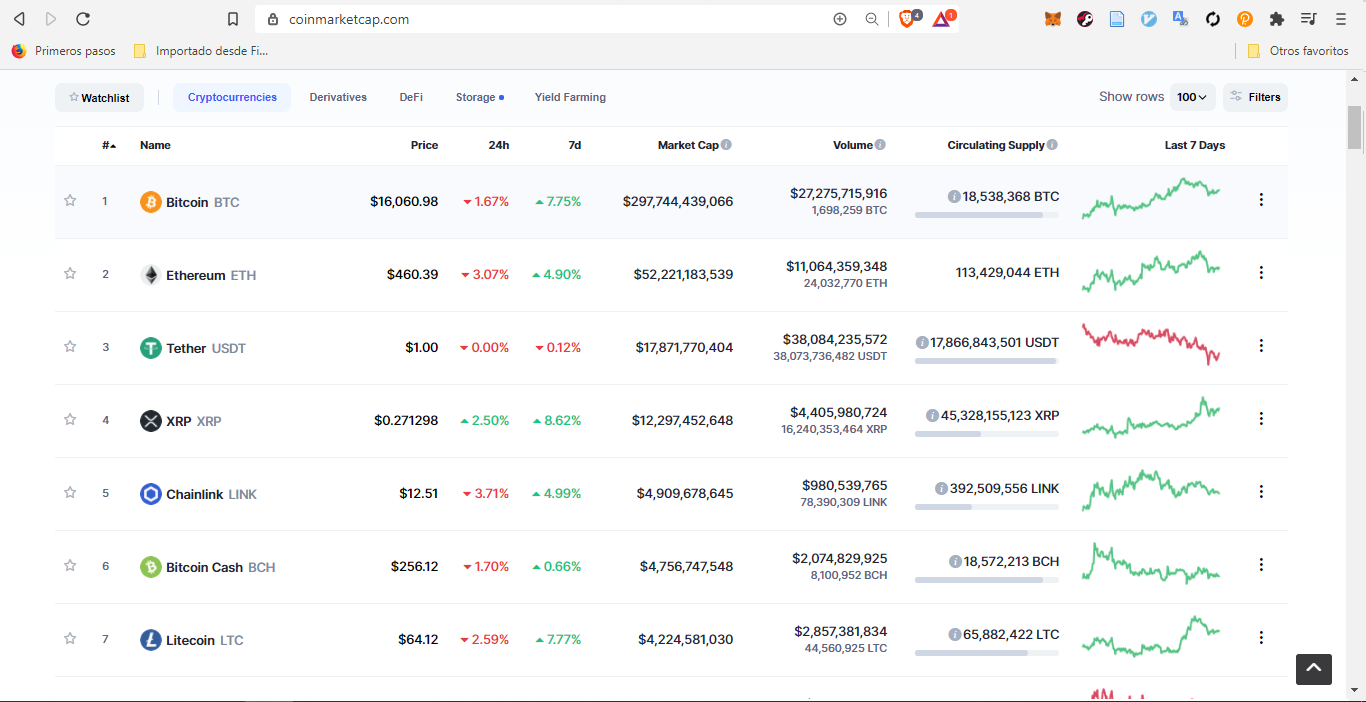
\includegraphics[scale=0.4]{coinmarketcap-valores.png}}
    \caption{Captura de pantalla de la  página CoinMarketCap el 14/11/2020 a las 21:23 hs Argentina} 
    \label{img:coinmarketcap-valores}
\end{figure}

\begin{figure}[hbt!]
    \centering
    {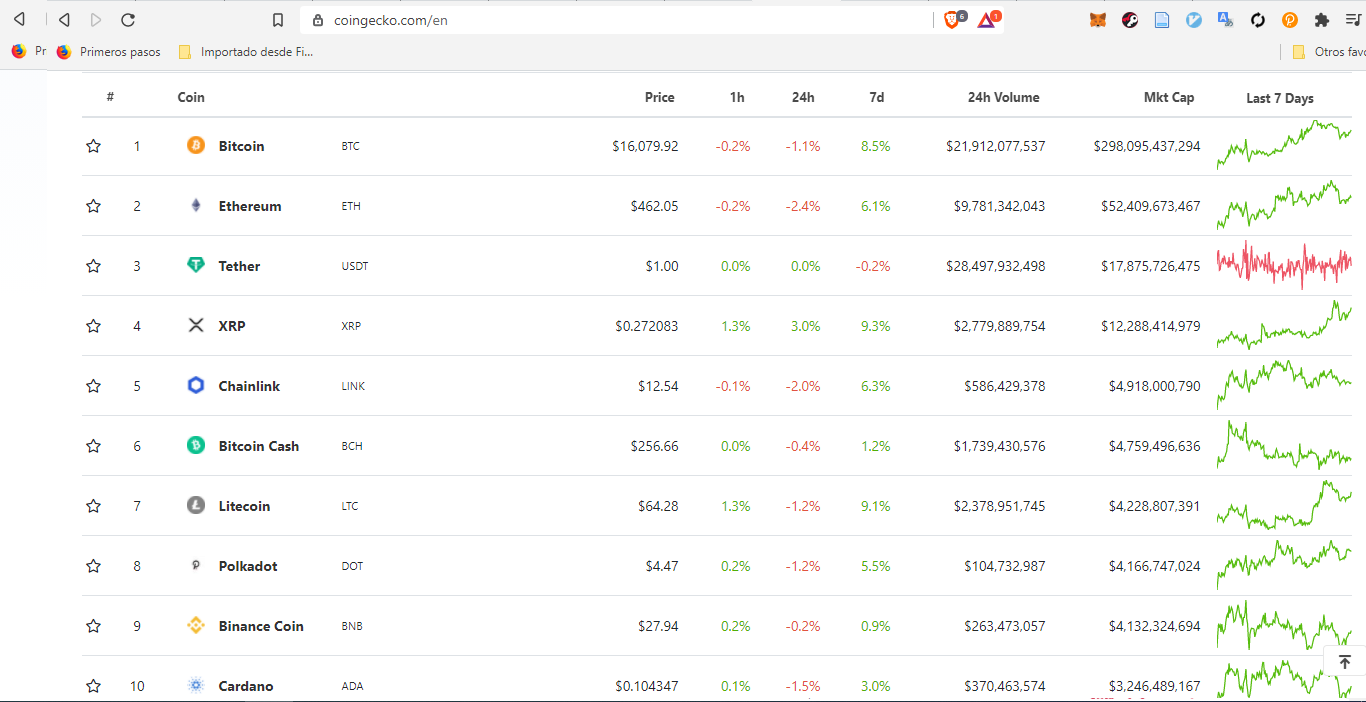
\includegraphics[scale=0.4]{coingecko-valores.png}}
    \caption{Captura de pantalla de la  página CoinGecko el 14/11/2020 a las 21:23 hs Argentina} 
    \label{img:coingecko-valores}
\end{figure}

En la  Figura \ref{img:coinmarketcap-valores} \footnote{Pagina Web CoinMarketCap: \url{https://coinmarketcap.com/}}  
de la página \pageref{img:coinmarketcap-valores} y 
Figura \ref{img:coingecko-valores}   \footnote{Pagina Web CoinGecko: \url{https://www.coingecko.com/en}}
de la página \pageref{img:coingecko-valores}  
muestra una lista de las \glsplural{criptomoneda} y los \glsplural{token} con mayor capital de mercado,
en los primeros dos puestos se observa el Bitcoin (BTC) y el Ether (ETH) que son criptomonedas nativas de sus Blockchain, 
en tercer lugar esta un token denominando Tether (USDT) que representa el valor del dolar, un USDT es igual a 
un dolar estadounidense, por lo menos esto pretende el proyecto en su whitepaper \cite[]{tether_tether_2016}, pero en la practica puede variar.
Asi como estas monedas digitales existen un sin numero de ellas y se crean constantemente, donde su valor reside en la oferta y demanda,
si no hay demanda por la obtención de un activo digital, no tiene valor \cite[]{joaquin_lopez_lerida_economiBlockchain_2016}.

\subsubsection{Tendencias Políticas}
Algunas de las noticias relacionados al gobierno Argentino, se impulsa un 
proyecto de ley para criptomonedas y activos digitales, donde buscan definir legalmente
esta tecnología para que el ecosistema local crezca, esto no es algo nuevo en el mundo
porque otros países como EE.UU., China , Rusia se encuentran operando con monedas digitales \cite[]{dagostino_exclusivo_nodate}.

